\documentclass[12pt, a4paper]{article}

\usepackage[T1]{fontenc}
\usepackage[utf8]{inputenc}


\usepackage[french]{babel} %Pour les langues
\PassOptionsToPackage{hyphens}{url}\usepackage{hyperref} %Pour les liens et les métadonnées
\usepackage[margin=2.5cm]{geometry} %Pour les marges de la page
\usepackage{mathtools} %Pour les maths
\usepackage{rotating} %Pour les figures penchées
\usepackage{siunitx} %Pour les unités

\hypersetup{
 colorlinks=true,
 linkcolor=black,
 urlcolor=blue,
 pdfauthor={Paul ROUSSEAU, Maxime BELLAUD, Gauthier L'ÉQUILBECQ, Khalil FALAH},
 pdftitle={Groupe 1 - Compte rendu}
} %Pour modifier la couleur des liens et définir les métadonnées

\allowdisplaybreaks %Pour avoir une suite d'équations sur plusieurs pages

\newcommand{\TInt}{\ensuremath{T_{int}}}
\newcommand{\TExt}{\ensuremath{T_{ext}}}
\newcommand{\hInt}{\ensuremath{h_{int}}}
\newcommand{\hExt}{\ensuremath{h_{ext}}}
\newcommand{\RUn}{\ensuremath{R_{1}}}
\newcommand{\RDeux}{\ensuremath{R_{2}}}
\newcommand{\RTrois}{\ensuremath{R_{3}}}
\newcommand{\RQuatre}{\ensuremath{R_{4}}}
\newcommand{\phiTot}{\ensuremath{\Phi_{tot}}}
\newcommand{\phiUn}{\ensuremath{\Phi_{1}}}
\newcommand{\phiDeux}{\ensuremath{\Phi_{2}}}
\newcommand{\phiTrois}{\ensuremath{\Phi_{3}}}
\newcommand{\phiQuatre}{\ensuremath{\Phi_{4}}}
\newcommand{\lambdaAlu}{\ensuremath{\lambda_{alu}}}
\newcommand{\lambdaVerre}{\ensuremath{\lambda_{verre}}}
\newcommand{\lambdaPlatre}{\ensuremath{\lambda_{platre}}}
\newcommand{\lambdaLDV}{\ensuremath{\lambda_{LDV}}}
\newcommand{\lambdaBeton}{\ensuremath{\lambda_{beton}}}
\newcommand{\lambdaCrepis}{\ensuremath{\lambda_{crepis}}}
\newcommand{\lambdaCarrel}{\ensuremath{\lambda_{carrel}}}
\newcommand{\ePlatre}{\ensuremath{e_{platre}}}
\newcommand{\eLDV}{\ensuremath{e_{LDV}}}
\newcommand{\eBeton}{\ensuremath{e_{beton}}}
\newcommand{\eCrepis}{\ensuremath{e_{crepis}}}
\newcommand{\eCarrel}{\ensuremath{e_{carrel}}}
\newcommand{\eAlu}{\ensuremath{e_{alu}}}
\newcommand{\eVerre}{\ensuremath{e_{verre}}}
\newcommand{\deltaT}{\ensuremath{\Delta T}}
\newcommand{\SCarrel}{\ensuremath{S_{carrel}}}
\newcommand{\SCrepis}{\ensuremath{S_{crepis}}}
\newcommand{\SAlu}{\ensuremath{S_{alu}}}
\newcommand{\SVerre}{\ensuremath{S_{verre}}}

\title{Transferts énergétiques - TP \\
Compte rendu}
\author{Groupe 1 : \\
Paul ROUSSEAU, Maxime BELLAUD, \\
Gauthier L'ÉQUILBECQ, Khalil FALAH}
\date{Mercredi 15 novembre 2023}

\begin{document}

\maketitle

\tableofcontents

\section{Introduction}

L'objectif de ce TP est de réaliser une étude des performances énergétiques du bâtiment G. Pour cela, la classe de TP étant séparé en quatre groupes, chacun réalise l'étude d'une face. Notre groupe, le groupe 1 réalisera l'étude pour la face Nord. Avec les résultats des autres groupes, nous pourront réaliser l'étude pour le bâtiment complet et enfin simuler le flux de chaleur pour différentes situations météorologiques (froid, chaud, neige, vent, etc...).

\section{Étude de la face Nord}

\subsection{Prise des mesures}

\subsection{Composition des murs et fenêtres}

Pour trouver les coefficients de conduction des différents matériaux, nous utilisons le document mis à disposition sur moodle «~JO-annexe\_4-th-bat.pdf~». Il se trouve également sur internet à l'adresse suivante : \url{https://www.novabuild.fr/sites/default/files/actualite/pdf/2021/08/re2020-arrete_du_4_aout_2021-annexe_4-th-bat.pdf}.

\paragraph{Fenêtres} \phantom{.} \\

Les fenêtres sont en simple vitrage (verre sodocalcique). Sur le document à la page 57, il est indiqué $\boxed{\lambdaVerre = \SI{1.00}{\watt\per\meter\per\kelvin}}$.

\paragraph{Bord des fenêtres} \phantom{.} \\

Les bords des fenêtres sont fait en aluminium. Le document indique à la page 77 que pour les menuiseries en aluminium, le coefficient de conductivité thermique est de $\boxed{\lambdaAlu = \SI{160}{\watt\per\meter\per\kelvin}}$.

\paragraph{Mur} \phantom{.} \\

Les murs sont plus complexes car ils sont composés de différents matériaux et il n'est évidemment pas possible d'ouvrir le mur pour voir ce qui le compose. Nous ferons donc des suppositions à l'aide de nos connaissance ainsi que des indications des professeurs. Ainsi, en partant de l'intérieur vers l'extérieur :

\begin{itemize}
\item Plâtre (Plâtre courant d’enduit intérieur), page 40 : $\boxed{\lambdaPlatre = \SI{0.57}{\watt\per\meter\per\kelvin}}$.
\item Laine de verre (abrégé en LDV), page 45 : $\boxed{\lambdaLDV = \SI{0.044}{\watt\per\meter\per\kelvin}}$. Nous choisissons la laine de verre avec une masse volumique comprise entre \SI{15}{\kilo\gram\per\meter\cubed} et \SI{20}{\kilo\gram\per\meter\cubed} car en recherchant quelques rouleaux de laine de verre sur internet,  les densités varient entre \SI{10}{\kilo\gram\per\meter\cubed} et \SI{30}{\kilo\gram\per\meter\cubed}.
\item Béton de structure, page 38 : $\boxed{\lambdaBeton = \SI{1.05}{\watt\per\meter\per\kelvin}}$. Nous choisissons le béton avec du sable de rivière et sans sable léger car c'est ce que nous pensons le plus courant.
\item Crépis (Mortier d'enduit), page 56 : $\boxed{\lambdaCrepis = \SI{1.30}{\watt\per\meter\per\kelvin}}$. Nous choisissons mortier d'enduit d'un masse volumique de \SI{1900}{\kilo\gram\per\meter\cubed} car c'est la valeur moyenne d'après le document (en bas du tableau).
\end{itemize}

\bigskip

À certains endroits, le mur est recouvert à l'extérieur d'un carrelage imitation brique. De même, d'après le site \href{https://fr.wikipedia.org/wiki/Grès_(céramique)}{https://fr.wikipedia.org/wiki/Grès\_(céramique)} ainsi que d'autres sites, il est précisé que les carrelages sont souvent fait en grès cérame. Le document indique à la page 35 $\boxed{\lambdaCarrel = \SI{2.30}{\watt\per\meter\per\kelvin}}$. Nous prenons cette valeur car c'est la valeur médiane des trois qui sont proposées.

\paragraph{Air} \phantom{.} \\

Le coefficient de convection thermique pour l'air n'est pas présent dans les documents fournis. Cependant, sur plusieurs site, par exemple \url{https://help.solidworks.com/2012/french/solidworks/cworks/Convection_Heat_Coefficient.htm}, il est indiqué que le coefficient de convection pour de l'air en convection naturelle se situe entre \SI{5}{\watt\per\meter\squared\per\kelvin} et \SI{25}{\watt\per\meter\squared\per\kelvin}. Après concertation avec notre professeur, nous prendrons $\boxed{\hInt = \SI{5}{\watt\per\meter\squared\per\kelvin} }$ et $\boxed{\hExt = \SI{25}{\watt\per\meter\squared\per\kelvin} }$

\subsection{Calcul du flux thermique}

On considère que le flux de chaleur est uniquement perpendiculaire au mur, c'est-à-dire que l'on néglige les flux allant du mur vers la vitre par exemple. Ainsi, on peut distinguer quatre cas possible pour les flux :

\begin{enumerate}
\item Le flux \phiUn\ passe par les vitres.
\item Le flux \phiDeux\ passe par le bord des fenêtres.
\item Le flux \phiTrois\ passe par le mur recouvert de crépis.
\item Le flux \phiQuatre\ passe par le mur recouvert de brique.
\end{enumerate}

En faisant une équivalence avec un circuit électrique, voici ce que nous obtenons sur la figure \ref{Schéma - équivalent} en annexe. On obtient ainsi l'égalité $\Phi = \phiUn + \phiDeux + \phiTrois + \phiQuatre$.

Avant de calculer les flux, commençons par calculer les résistances thermiques équivalentes de chaque branche : 

\bigskip

\begin{align*}
 & \RUn  = \frac{1}{\hInt} + \frac{\ePlatre}{\lambdaPlatre} + \frac{\eLDV}{\lambdaLDV} + \frac{\eBeton}{\lambdaBeton} + \frac{\eCrepis}{\lambdaCrepis} + \frac{\eCarrel}{\lambdaCarrel} + \frac{1}{\hExt} \\ \\
 & \RUn = \frac{1}{5} + \frac{\num{12.5e-3}}{0.57} + \frac{\num{6.5e-2}}{0.044} + \frac{\num{20e-2}}{1.05} + \frac{\num{1e-2}}{1.30} + \frac{\num{7e-3}}{2.30} + \frac{1}{25} \\ \\
 & \boxed{\RUn = \SI{1.94}{\meter\squared\kelvin\per\watt}} \\ \\
 & \RDeux  = \frac{1}{\hInt} + \frac{\ePlatre}{\lambdaPlatre} + \frac{\eLDV}{\lambdaLDV} + \frac{\eBeton}{\lambdaBeton} + \frac{\eCrepis}{\lambdaCrepis} + \frac{1}{\hExt} \\ \\
 & \RDeux = \frac{1}{5} + \frac{\num{12.5e-3}}{0.57} + \frac{\num{6.5e-2}}{0.044} + \frac{\num{20e-2}}{1.05} + \frac{\num{1e-2}}{1.30} + \frac{1}{25} \\ \\
 & \boxed{\RDeux = \SI{1.94}{\meter\squared\kelvin\per\watt}} \\ \\
 & \RTrois  = \frac{1}{\hInt} + \frac{\eAlu}{\lambdaAlu} + \frac{1}{\hExt} \\ \\
 & \RTrois = \frac{1}{5} + \frac{\num{2.8e-2}}{160} + \frac{1}{25} \\ \\
 & \boxed{\RTrois = \SI{0.24}{\meter\squared\kelvin\per\watt}} \\ \\
 & \RQuatre  = \frac{1}{\hInt} + \frac{\eVerre}{\lambdaVerre} + \frac{1}{\hExt} \\ \\
 & \RQuatre = \frac{1}{5} + \frac{\num{1.4e-2}}{1.00} + \frac{1}{25} \\ \\
 & \boxed{\RQuatre = \SI{0.25}{\meter\squared\kelvin\per\watt}}
\end{align*}

\bigskip

La loi d'Ohm en électricité est $U = R \times I$. $U$ est une tension, c'est-à-dire une différence de potentiel. Dans notre cas, le $U$ devient une différence de température notée $\deltaT = \TInt - \TExt$. $R$ est une résistance et ne change pas entre la loi électrique et notre cas. Finalement, $I$ est un flux d'électrons, ce qui signifie que cela correspond à nos flux $\Phi$. Il faut penser à prendre en compte la surface $S$ et on a alors : $\deltaT = \frac{R \times \Phi}{S}$, ce qui devient $\Phi = \frac{\deltaT \times S}{R}$.

Dans notre cas, on prend $\TInt = \SI{22}{\degree C}$ et $\TExt = \SI{11}{\degree C}$ (d'après Météo France). Cela fait donc $\deltaT = 22 - 11 = \boxed{11 = \deltaT}$.

\begin{align*}
 & \phiUn = \frac{\deltaT \times \SCarrel}{\RUn} \\ \\
 & \phiUn = \frac{11 \times 0.65}{1.94} \\ \\
 & \boxed{\phiUn = \SI{3.69}{\watt}} \\ \\
 & \phiDeux = \frac{\deltaT \times \SCrepis}{\RDeux} \\ \\
 & \phiDeux = \frac{11 \times 3.5}{1.94} \\ \\
 & \boxed{\phiDeux = \SI{19.85}{\watt}} \\ \\
 & \phiTrois = \frac{\deltaT \times \SAlu}{\RTrois} \\ \\
 & \phiTrois = \frac{11 \times 1.04}{0.24} \\ \\
 & \boxed{\phiTrois = \SI{47.67}{\watt}} \\ \\
 & \phiQuatre = \frac{\deltaT \times \SVerre}{\RQuatre} \\ \\
 & \phiQuatre = \frac{11 \times 2.54}{0.25} \\ \\
 & \boxed{\phiQuatre = \SI{111.76}{\watt}}
\end{align*}

\bigskip

Finalement :

\begin{align*}
 & \Phi = \phiUn + \phiDeux + \phiTrois + \phiQuatre \\ \\
 & \Phi = 3.69 + 19.85 + 47.67 + 111.76 \\ \\
 & \boxed{\Phi = \SI{182.97}{\watt}}
\end{align*}

\bigskip

On rappelle que l'on a fait cette étude uniquement au sous-sol, qui est à moitié enterré dans la terre, ce que l'on a négligé. La surface des murs au rez-de-chaussée est environ deux fois plus grande que la surface des murs que l'on a considéré pour le sous-sol. De plus, les matériaux sont similaires et la proportion de carrelage n'a pas d'influence car avec les approximations, les résistances avec ou sans le carrelage sont identiques. De même, la surface de fenêtre est proportionnellement similaire. Nous calculerons donc le flux total de la face nord en triplant le flux du sous-sol :

\begin{align*}
 & \phiTot = 3 \times \Phi \\ \\
 & \phiTot = 3 \times 182.97 \\ \\
 & \boxed{\phiTot = \SI{548.91}{\watt}} \\ \\
\end{align*}

\section{Étude du bâtiment complet}

\section{Étude pour différentes situations}

\subsection{Température extérieure de -10°C, temps sec}

\subsection{Température extérieure de -10°C avec une couche de neige sur le toit de 20cm}

\subsection{Température extérieure de +40°C}

\subsection{Température extérieure de +10°C avec 100 km/h de vent}

\section{Conclusion}

\newpage

\phantom{.}
\vfill
\centering

\section{Annexes}

\vfill

\newpage

\begin{sidewaysfigure}
 \centering
 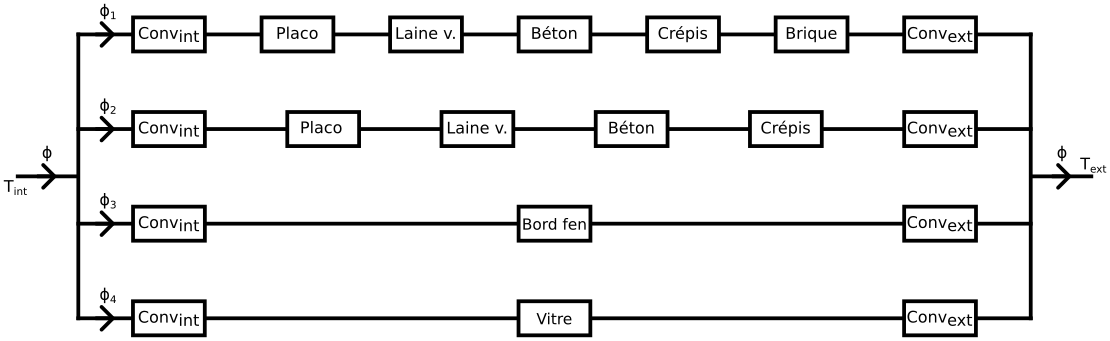
\includegraphics[width=\textwidth]{Schémas/Schéma - Équivalence électrique.png}
 \caption{Schéma électrique équivalent.}
 \label{Schéma - équivalent}
\end{sidewaysfigure}

\end{document}
